% !TEX TS-program = pdflatex
% !TEX encoding = UTF-8 Unicode

% This is a simple template for a LaTeX document using the "article" class.
% See "book", "report", "letter" for other types of document.

\documentclass[11pt]{article} % use larger type; default would be 10pt

\usepackage[utf8]{inputenc} % set input encoding (not needed with XeLaTeX)

%%% Examples of Article customizations
% These packages are optional, depending whether you want the features they provide.
% See the LaTeX Companion or other references for full information.

%%% PAGE DIMENSIONS
\usepackage{geometry} % to change the page dimensions
\geometry{a4paper} % or letterpaper (US) or a5paper or....
% \geometry{margin=2in} % for example, change the margins to 2 inches all round
% \geometry{landscape} % set up the page for landscape
%   read geometry.pdf for detailed page layout information

\usepackage{graphicx} % support the \includegraphics command and options
\usepackage{topcapt}

% \usepackage[parfill]{parskip} % Activate to begin paragraphs with an empty line rather than an indent

%%% PACKAGES
\usepackage{booktabs} % for much better looking tables
\usepackage{array} % for better arrays (eg matrices) in maths
\usepackage{paralist} % very flexible & customisable lists (eg. enumerate/itemize, etc.)
\usepackage{verbatim} % adds environment for commenting out blocks of text & for better verbatim
\usepackage{subfig} % make it possible to include more than one captioned figure/table in a single float
% These packages are all incorporated in the memoir class to one degree or another...

%%% HEADERS & FOOTERS
\usepackage{fancyhdr} % This should be set AFTER setting up the page geometry
\pagestyle{fancy} % options: empty , plain , fancy
\renewcommand{\headrulewidth}{0pt} % customise the layout...
\lhead{}\chead{}\rhead{}
\lfoot{}\cfoot{\thepage}\rfoot{}

%%% SECTION TITLE APPEARANCE
\usepackage{sectsty}
\allsectionsfont{\sffamily\mdseries\upshape} % (See the fntguide.pdf for font help)
% (This matches ConTeXt defaults)

%%%% ToC (table of contents) APPEARANCE
%\usepackage[nottoc,notlof,notlot]{tocbibind} % Put the bibliography in the ToC
%\usepackage[titles,subfigure]{tocloft} % Alter the style of the Table of Contents
%\renewcommand{\cftsecfont}{\rmfamily\mdseries\upshape}
%\renewcommand{\cftsecpagefont}{\rmfamily\mdseries\upshape} % No bold!

%%% END Article customizations

%%% The "real" document content comes below...

\title{Differential gene expression in males vs females for head and neck squamous cancers (HNSC)}
\author{Czuee Morey}
%\date{} % Activate to display a given date or no date (if empty),
         % otherwise the current date is printed 

\begin{document}
\maketitle

The gene expression data for HNSC was taken from the Cancer genome atlas study \cite{nature}. The data contained 566 samples for RNA-seq from males and females. In some cases, normal samples from the same individual were also present. The data was treated suitably for analysis. In part 1, the normal tissues were removed and only tumor samples were considered. In part 2, the samples for which both tumor and normal tissue are present were considered. The log of gene expression(+1) was considered for all cases, and the expression was centered around the mean in some cases.

\begin{figure}[htbp]
\centering
\subfloat{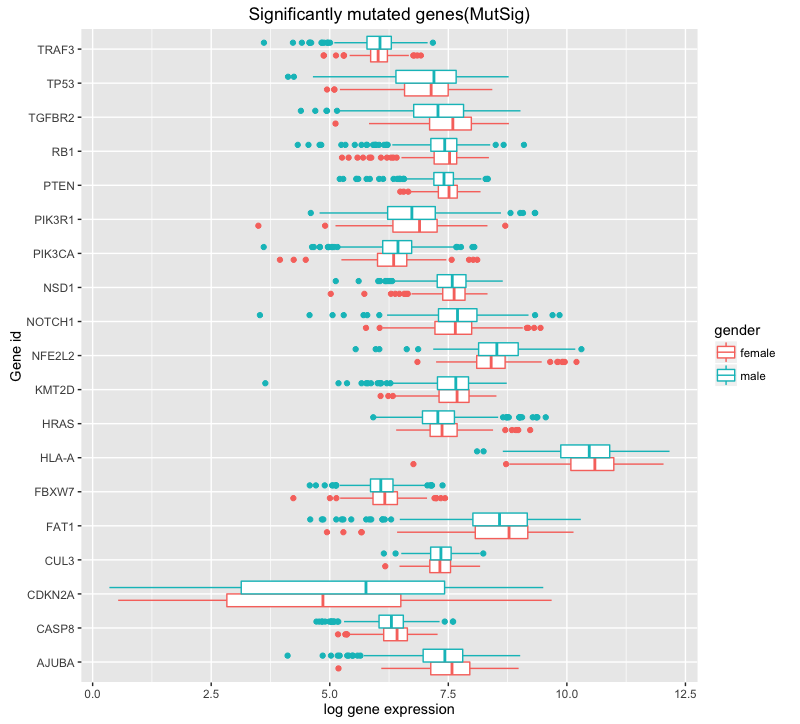
\includegraphics[width=0.5\textwidth]{Plots/Expression_mutsig_genes.png}}
\subfloat{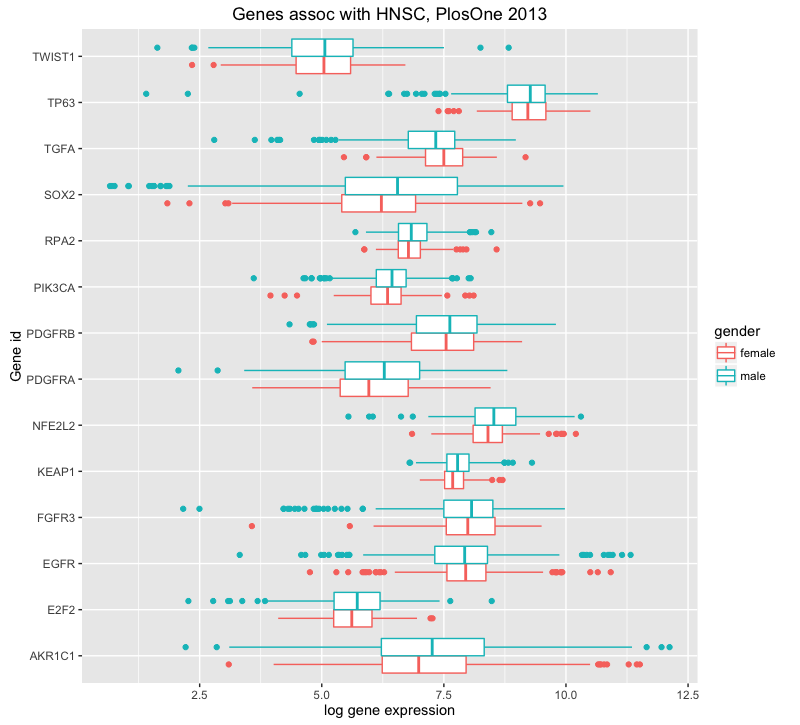
\includegraphics[width=0.5\textwidth]{Plots/Exp_HNSC-genes_Pone.png}}
\caption{Significantly mutated genes \cite{nature} and genes associated with HNSC \cite{pone} do not show differential expression between males and females.}
\label{mutsig}
\end{figure}

\section{Difference in gene expression between tumor samples from males vs females. }

\subsection{Selecting genes with highest variability}

The genes were filtered to select only genes that would have the highest variance in their gene expression and are more likely to have differential expression between males and females. The genes were sorted by the standard deviation (SD) of gene expression from all samples. The figure~\ref{sd-plot} shows the plot with ordered

\begin{figure}[htbp]
\centering
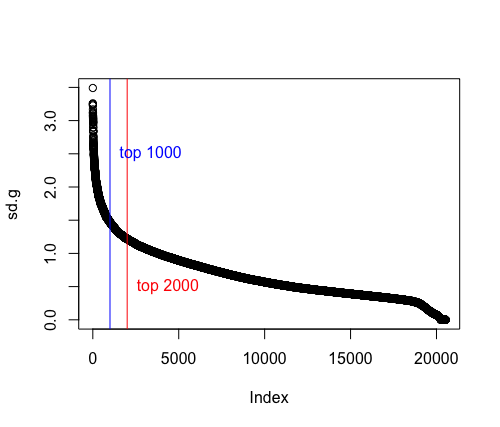
\includegraphics[width=0.5\textwidth]{Plots/SD-plot_top1k2k.png}
\caption{Plot for Standard deviation of gene expression ordered from highest to lowest. The vertical lines indicate the position for first 1000 and 2000 genes that were selected for further study.}
\label{sd-plot}
\end{figure}

\subsection{Genes with significant difference in means between males and females}

\begin{figure}[htbp]
\centering
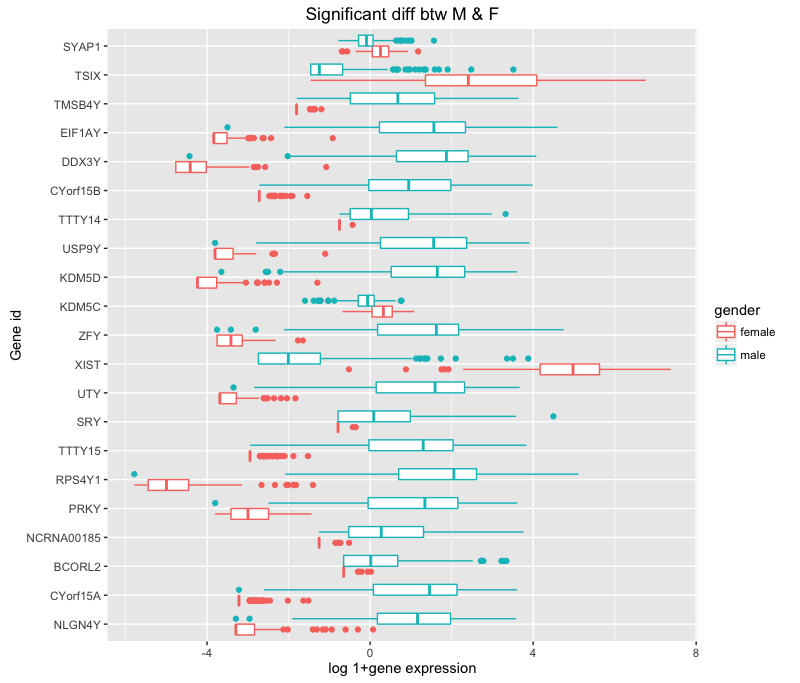
\includegraphics[width=0.5\textwidth]{Plots/Signif21_genenames_boxplot.png}
\caption{The genes that have a difference between their means in males and females greater than the SD of the entire distribution were selected. 21 genes were found.}
\label{diff-mean}
\end{figure}

\begin{table}[htbp]
   \centering
   \caption{The genes that have a difference between their means in males and females greater than the SD of the entire distribution were selected. 19 descriptions - NCRNA00185 and TTTY14 are the same gene. Also CYorf15A and B have the same description. All the genes are X and Y linked only.} % requires the topcapt package
   \begin{tabular}{p{1.5cm} p{10cm} p{2.5cm}} % Column formatting, @{} suppresses leading/trailing space
   \toprule
Approved Symbol & Approved Name & Chromosome \\
\midrule
DDX3Y & DEAD-box helicase 3, Y-linked & Yq11 \\
EIF1AY & eukaryotic translation initiation factor 1A, Y-linked & Yq11.223 \\
KDM5C & lysine demethylase 5C & Xp11.22-p11.21 \\
KDM5D & lysine demethylase 5D & Yq11 \\
NLGN4Y & neuroligin 4, Y-linked & Yq11.221 \\
PRKY & protein kinase, Y-linked, pseudogene & Yp11.2 \\
RPS4Y1 & ribosomal protein S4, Y-linked 1 & Yp11.3 \\
SRY & sex determining region Y & Yp11.3 \\
SYAP1 & synapse associated protein 1 & Xp22.31 \\
TMSB4Y & thymosin beta 4, Y-linked & Yq11.221 \\
TSIX & TSIX transcript, XIST antisense RNA & Xq13.2 \\
TTTY14 & testis-specific transcript, Y-linked 14 (non-protein coding) & Yq11.222 \\
TTTY15 & testis-specific transcript, Y-linked 15 (non-protein coding) & Yq11.1 \\
USP9Y & ubiquitin specific peptidase 9, Y-linked & Yq11.2 \\
UTY & ubiquitously transcribed tetratricopeptide repeat containing, Y-linked & Yq11.221 \\
XIST & X inactive specific transcript (non-protein coding) & Xq13.2 \\
ZFY & zinc finger protein, Y-linked & Yp11.3 \\

\bottomrule
   \end{tabular}
   \label{tab:itc}
\end{table}

\begin{thebibliography}{9}

\bibitem{nature} 
Network, T. C. G. A. (2015)
\textit{Comprehensive genomic characterization of head and neck squamous cell carcinomas}. 
Nature 517, 576–582.

\bibitem{pone}
Vonn Walter et al (2013)
\textit{Molecular Subtypes in Head and Neck Cancer Exhibit
Distinct Patterns of Chromosomal Gain and Loss of
Canonical Cancer Genes}
Plos One 8(2), e56823.

\end{thebibliography}
\end{document}
